\section{Application}

  This section will explore the application of the aforementioned software
  engineering techniques to the development of the software used for Mariokart.

  \subsection{Version Control}

    The version control system used for this project was Git.  The reasons for
    choosing this over something else like SVN or Hg were:

    \begin{itemize}
      \item DVCS are the way of the future.  There is almost nothing that SVN
      does better than Git or Hg, the few things it does are niche features such
      as being able to checkout just a sub folder in the repository.

      \item Two of the developers on the project had previously used Git and
      were using it daily for many other projects.

      \item GitHub provided us with many very useful features such as a Wiki to
      use for documentation and project management.
    \end{itemize}

    This turned out to be a very good choice, some of the major positives were:

    \begin{itemize}
      \item The wiki, throughout the project we recorded details on our
      decisions on the wiki.  This has proven invaluable now when looking back
      we have to figure out details such as why exactly we chose the SAM7XC.

      \item Painless branching and merging.  This was very helpful at a few
      points during the development; at one point it was decided that the Atmel
      CAN library was untrustworthy and would require a rewrite.  While that was
      going on in a different branch the rest of the development could continue
      on in the main branch.  Once the module was re-written it was simple to
      merge it back in and change the few cases where the interface had changed.
      Also, when we were coming up to give a demonstration it was easy enough
      for each member to branch off and write their demo code in their own
      branch, this ensured that any changes they had to make to ensure the demo
      went smoothly could be segregated.

      \item CI Joe integration, this will be detailed more later, but the
      combination of Git and GitHub made it extremely simple to set up CI Joe.
    \end{itemize}

  \subsection{Unit Testing}

    Unfortunately this was not implemented in our project.  The possibility of
    implementing it was explored, but the lack of time prevented it from
    continuing.

  \subsection{Continuous Integration}

    Continuous integration was implemented using a piece of software known as CI
    Joe.  This is a continuous integration server designed to be as simple as
    possible to setup \cite{ci-joe}.  You provide CI Joe with a git repository and a command
    to use to test the project and you are done.  In our case since we did not
    have the time to set up a unit testing system we just had CI Joe building
    the project to detect any compilation errors or warnings.

    Once the basics of CI Joe were set up a few more complex things could very
    easily be done with it.  The trigger to tell it to update and attempt a new
    build was a simple HTTP POST, GitHub supported POST-hooks to notify services
    when someone pushed code to the repository, so we could easily add a link to
    CI Joe with that.  This meant that every time somebody changed anything CI
    Joe would run.

    The next step was getting the output from Joe, the basic interface was via a
    website as shown in Figure \ref{joe-website}.  Additionally to this we were
    able to set up a build-hook that would be run when the build was finished.
    This was setup to push the status of the build to a dashboard so we could
    utilise multiple instances of CI Joe for different projects (shown in Figure
    \ref{joe-dashboard}) along with sending an email out to the group mailing
    list when a failure occurred (shown in Figure \ref{joe-email}).

    \begin{figure}
    \centering
    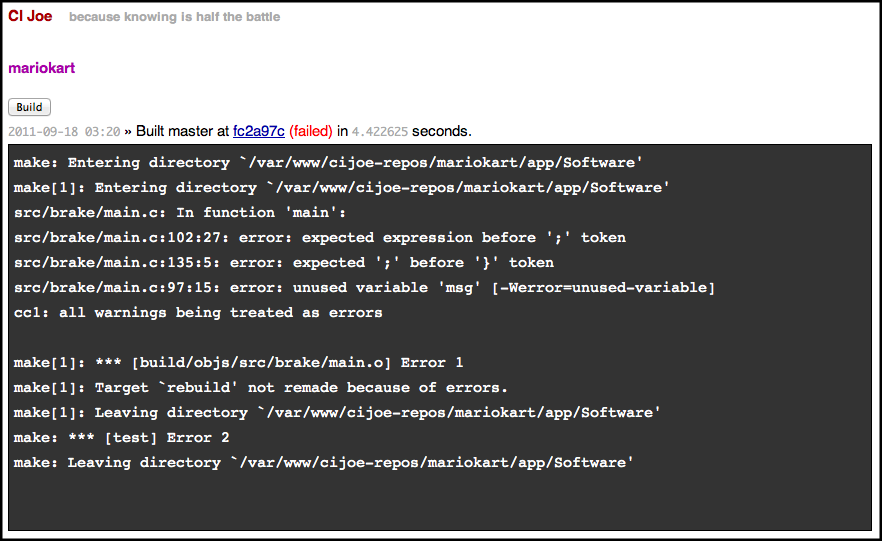
\includegraphics[width=0.45\textwidth]{images/joe-website}
    \caption{CI Joe's website interface.}
    \label{joe-website}
    \end{figure}

    \begin{figure}
    \centering
    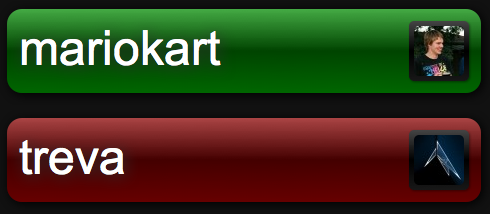
\includegraphics[width=0.3\textwidth]{images/joe-dashboard}
    \caption{Dashboard set up to show multiple CI Joes statuses.}
    \label{joe-dashboard}
    \end{figure}

    \begin{figure}
    \centering
    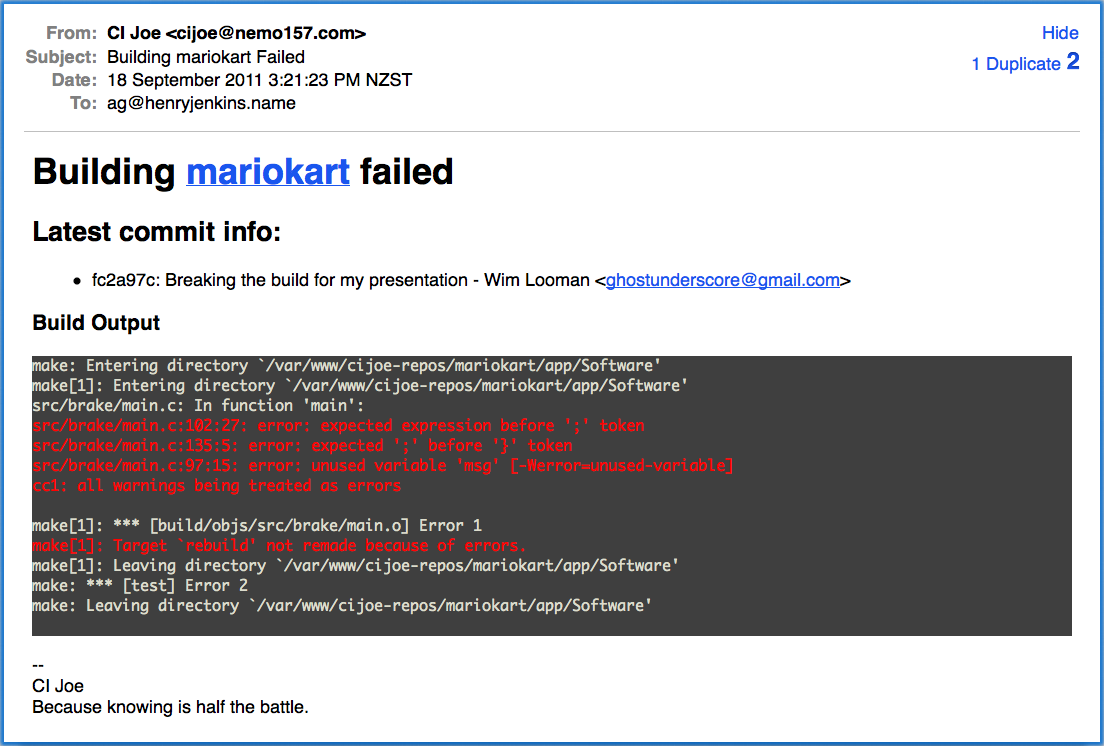
\includegraphics[width=0.45\textwidth]{images/joe-email}
    \caption{Build failure email from CI Joe.}
    \label{joe-email}
    \end{figure}
